\documentclass[11pt,a4paper]{IEEEtran}
\usepackage[ngerman]{babel}
\usepackage[utf8]{inputenc}
\usepackage{enumitem} % referencable enumerations
\usepackage{eurosym}

\usepackage[binary-units=true]{siunitx}
% make inches available as a unit
\let\DeclareUSUnit\DeclareSIUnit
\let\US\SI \DeclareUSUnit\inch{Zoll}

\usepackage{biblatex}
\addbibresource{references.bib}
\usepackage{tikz}
\usetikzlibrary{shapes, shapes.geometric, arrows, automata}
\usepackage{adjustbox}

\begin{document}

\title{DIY-Projekt Kaffeekasse} \author{\IEEEauthorblockN{Martin Hofmann}\\
\IEEEauthorblockA{Universität Erlangen-Nürnberg\\ Email: martin.hofmann@fau.de}
}

\date{6. Februar 2016}

\maketitle \begin{abstract} Blubbblabla \end{abstract}

\section{Motivation}

Ziel des Projektes ist es, ein System zur Verwaltung von Nutzerkonten und zur
Abrechnung von 

Um die Abrechnung von Kaffeekäufen einfach zu gestalten, ergaben sich folgende
Anforderungen an das System:

\begin{enumerate} 
    \item\label{req0} Die Authentifizierung von Nutzern muss
        einfach erfolgen.  
    \item\label{req1} Die Bedienung des Gerätes muss
        intuitiv möglich sein.  
    \item\label{req2} Das Gerät muss ohne
        Netzwerkverbindung funktionieren.  
\end{enumerate}

Anforderung \ref{req0} soll durch die Verwendung von Firmenausweisen zur
Identifizierung von Nutzern gelöst werden. Neben technischen Schwierigkeiten,
auf die im Kapitel \ref{sec:rfid} genauer eingegangen wird, ergaben sich
hierbei auch den Datenschutz betreffende Konsequenzen.

Beim Zugriff auf den Firmenausweis soll das Lesen von persönlichen
Informationen (Personalnummer, Schließberechtigungen und ähnliches)
unterbleiben. Da im Rahmen dieses Projektes jedoch nur die ID-Nummer des im
Ausweis eingebetteten Chips benötigt wird, welche nicht ohne weiteres der
Personalnummer zugeordnet werden kann, sind datenschutztechnische Belange
erfüllt.

Um eine einfache Bedienung des Gerätes nach Punkt \ref{req1} zu ermöglichen,
wurde entschieden, eine Touch-Oberfläche zu entwickeln. Auf Details hierzu wird
in den Kapiteln \ref{sec:hw} (der verwendete Touchscreen) und \ref{sec:sw}
(Software für die grafische Oberfläche) eingegangen.

\section{Auslesen von RFID-Karten} \label{sec:rfid}

Die Abkürzung RFID steht für \emph{radio-frequency identification} und
beschreibt allgemein das Verwenden von Funksystemen zur Identifizierung. Eine
Untermenge von RFID ist NFC (\emph{near-field communication},
Nahfeldkommunikation), welches den Frequenzbereich von \SI{13,56}{\mega\hertz}
benutzt.

\begin{figure}[ht]
    \label{fig:rfid125khz}
    \centering
    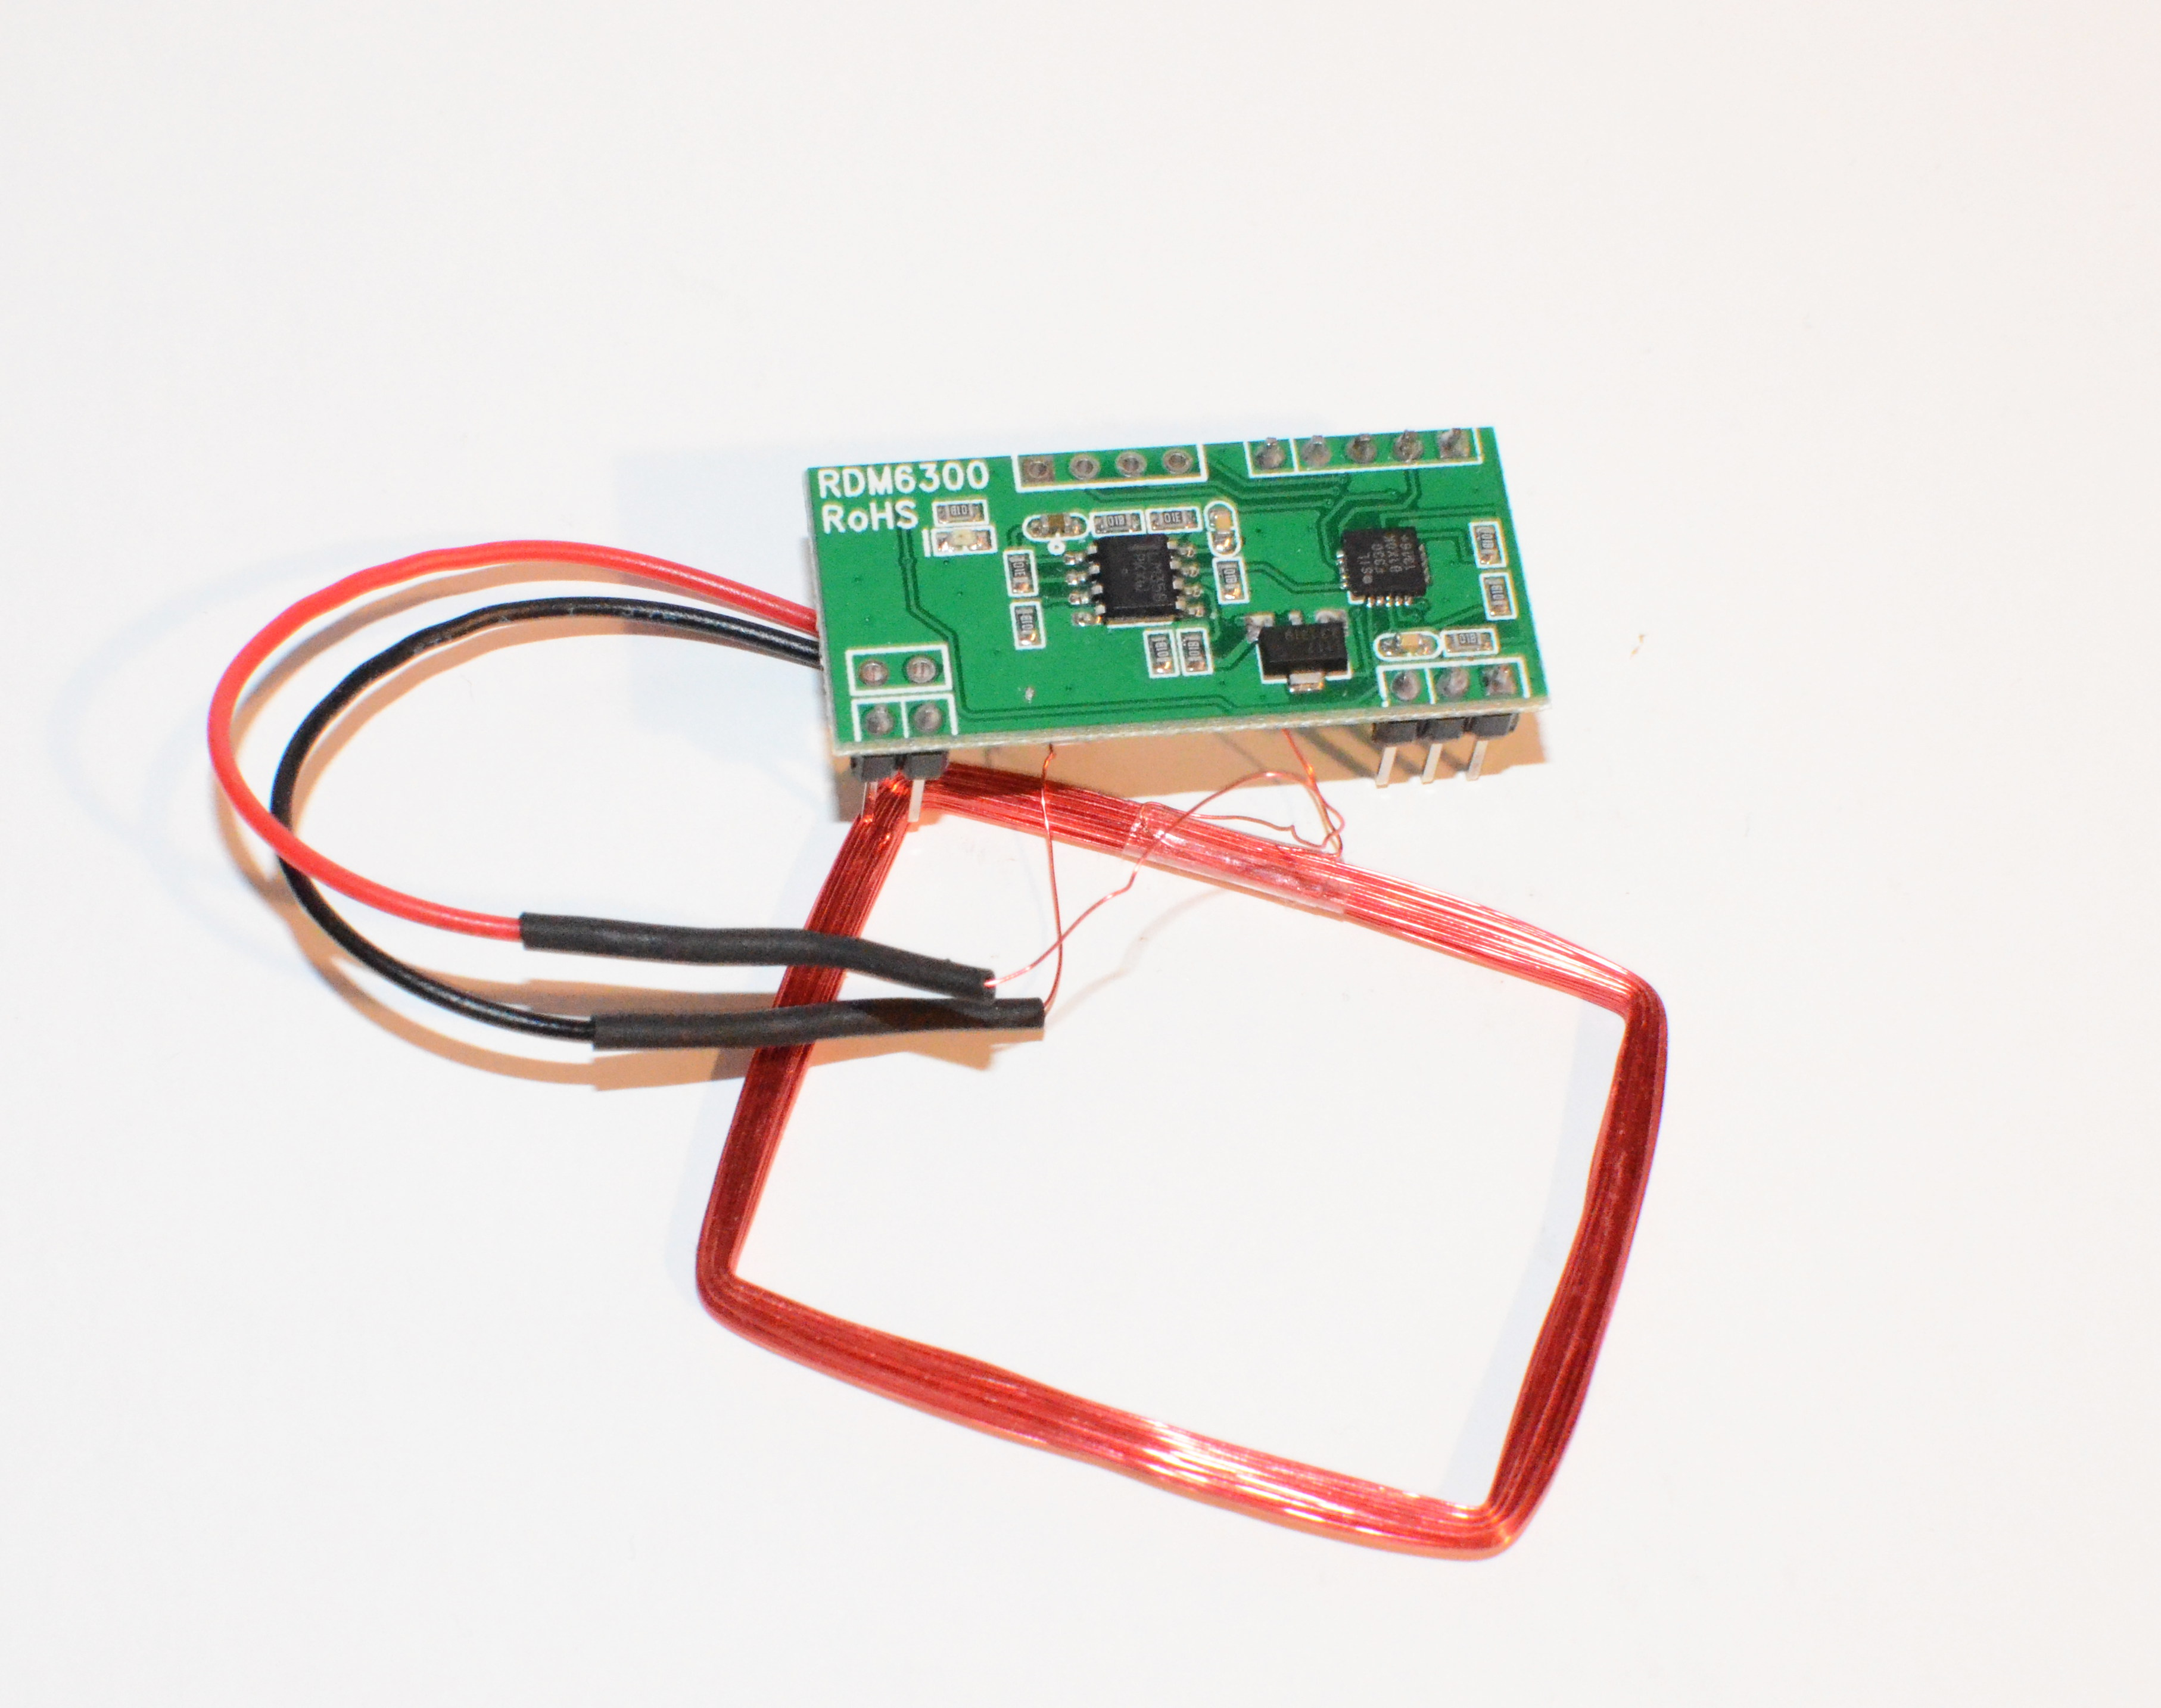
\includegraphics[width=.8\columnwidth]{images/125khz_rfid}
    \caption{RFID-Modul für \SI{125}{\kilo\hertz}}
\end{figure}

Im DIY-Bereich sind verschiedene RFID-Module für populäre Plattformen wie
Arduino oder den Raspberry Pi erhältlich. Da zu Beginn unbekannt war, welchen
Frequenzbereich in den ID-Karten verwendet wird, wurde zuerst ein 
\SI{125}{\kilo\hertz} Modul ausprobiert (siehe Abbildung \ref{fig:rfid125khz}).
Dieses erkannte die gewünschten Karten jedoch nicht. 

\begin{figure}[ht]
    \label{fig:rfidnfc}
    \centering
    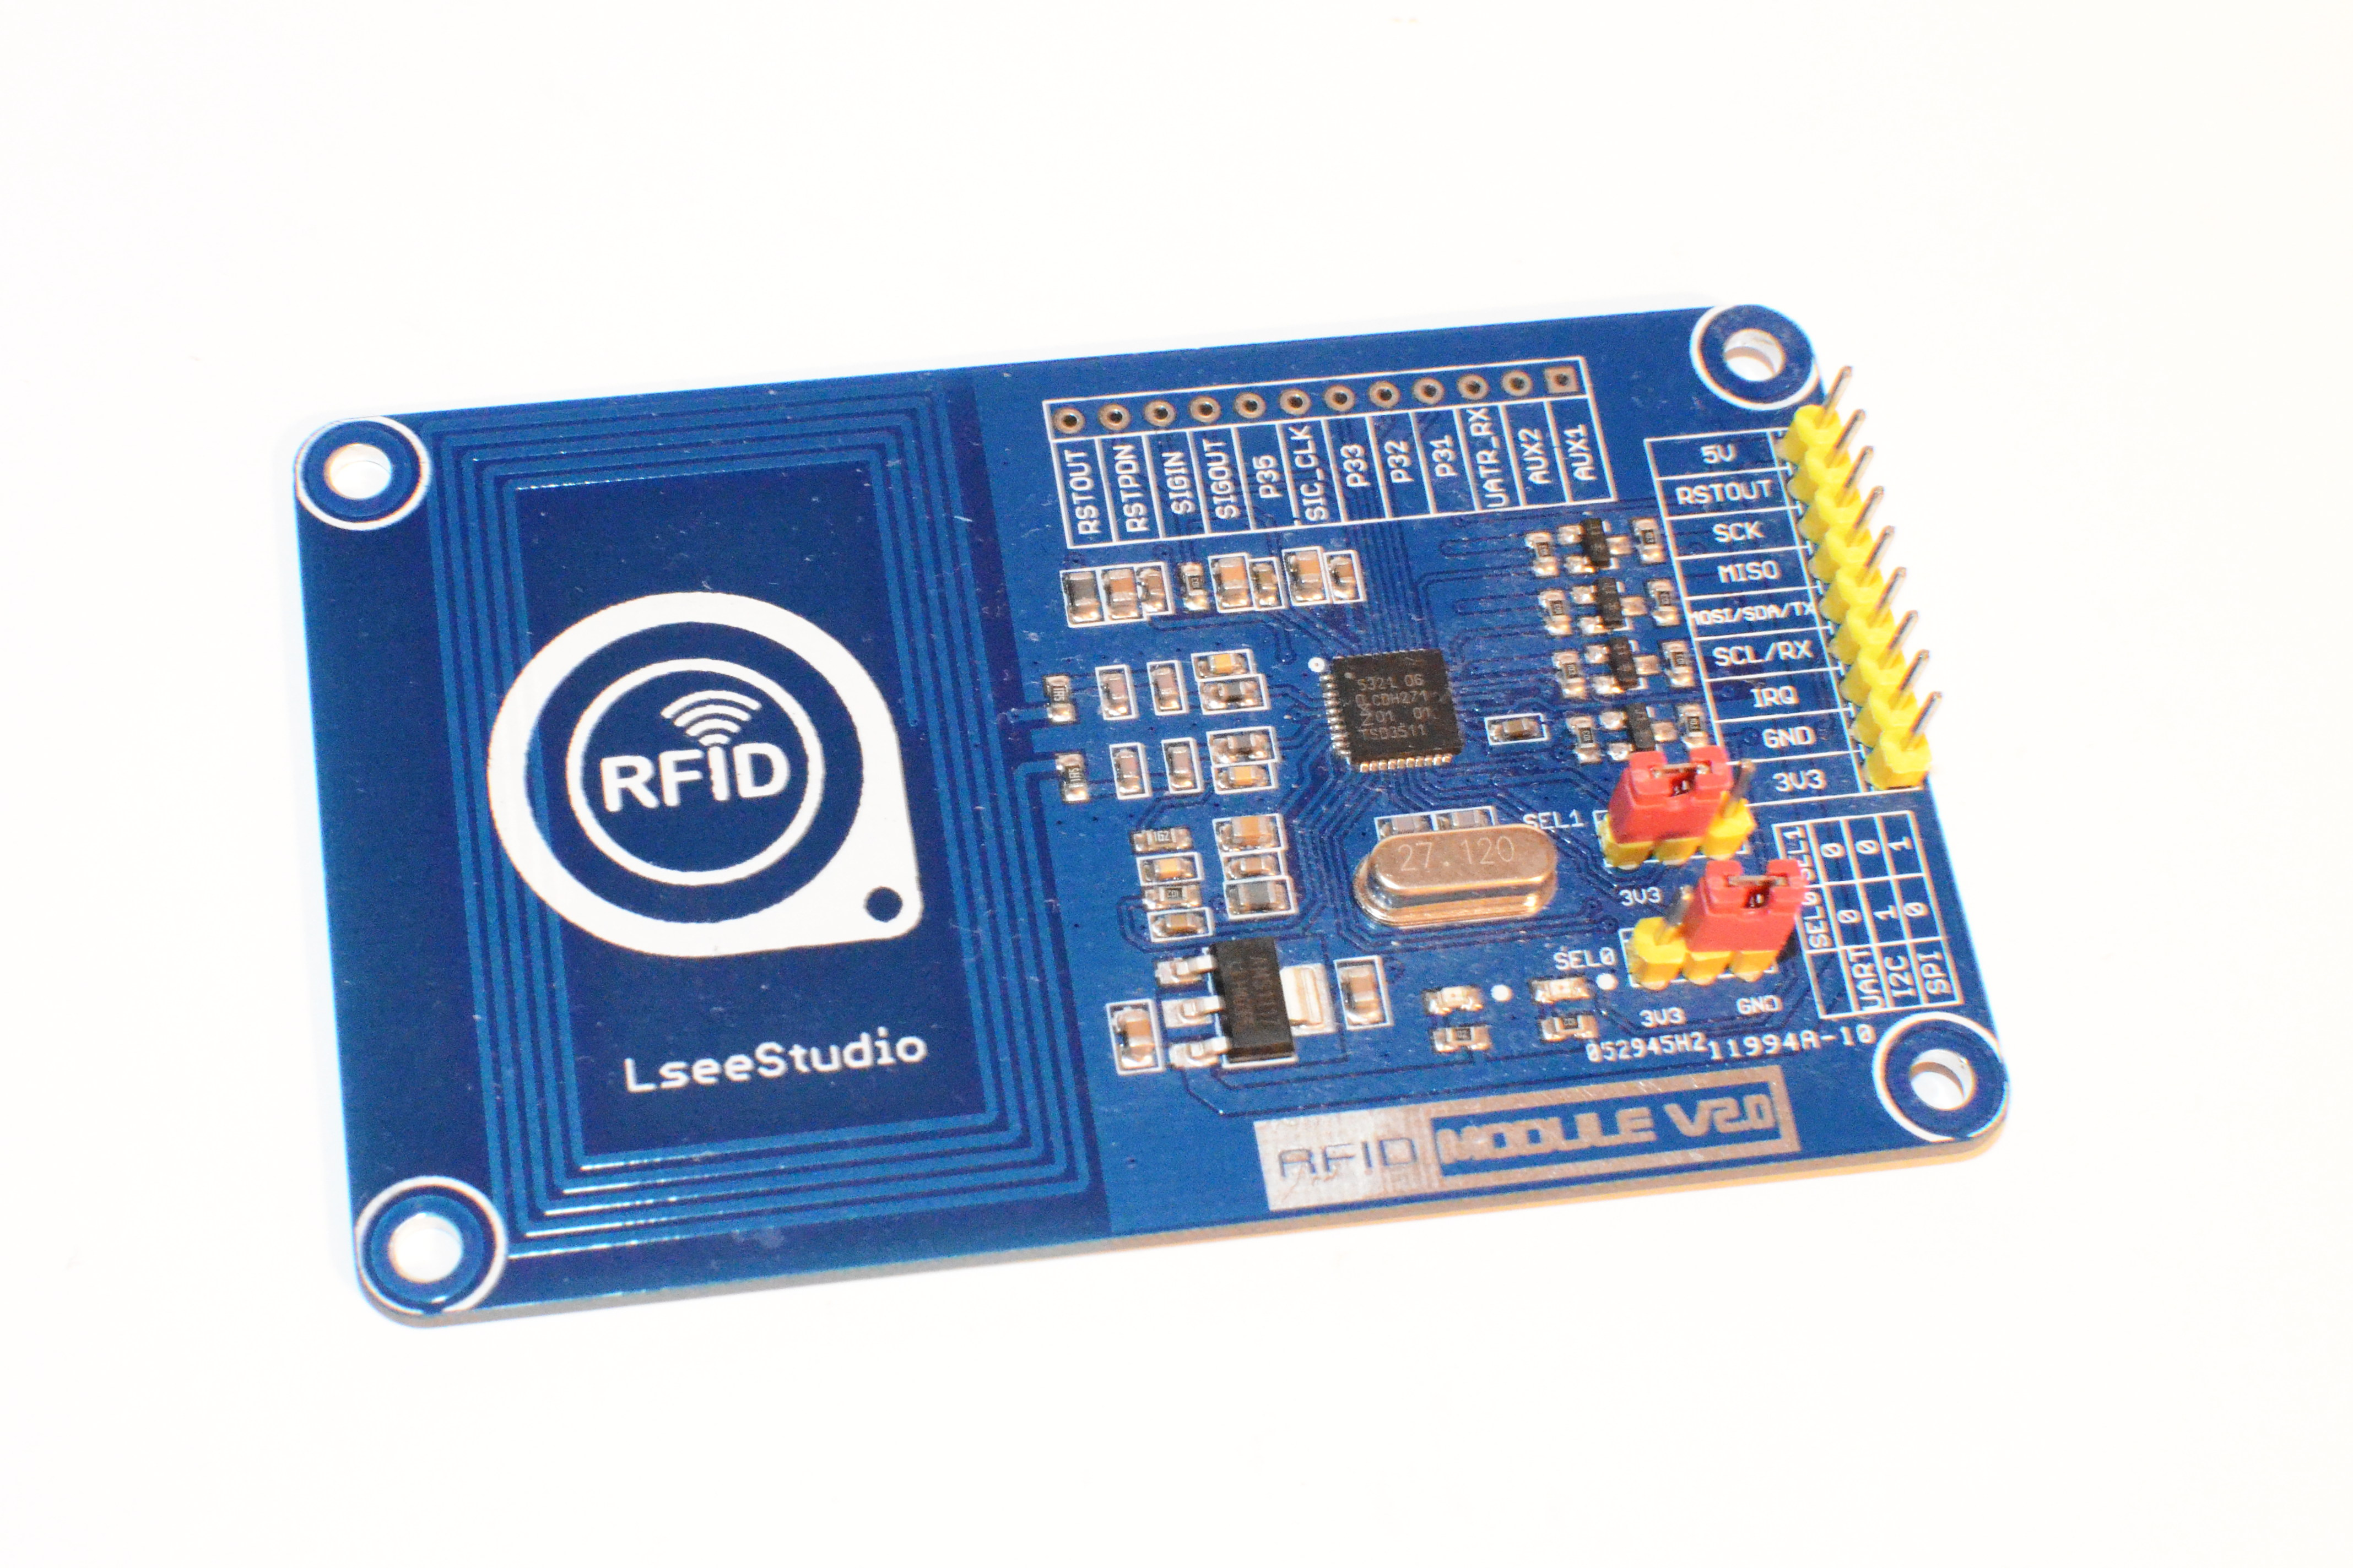
\includegraphics[width=.8\columnwidth]{images/nfc_reader}
    \caption{RFID-Modul für NFC}
\end{figure}

Häufig werden zu Identifikationszwecken Chipkarten der Marke \emph{Mifare} nach
dem NFC-Standard verwendet, so auch in den Studierendenausweisen der
FAU\autocite{FauCARD}. Es erschien deshalb logisch, als nächsten Schritt ein
entsprechendes Lesegerät zu testen. Das Auslesen dieser Karten ist mit dem
PN532-Mikrocontroller von NXP möglich. Der Chip ist von der amerikanischen
Firma Adafruit\autocite{AdafruitHP} auf einer Platine samt Anschlüssen und
Antenne erhältlich (siehe Abbildung \ref{fig:rfidnfc}).

Der PN532 kann an den Raspberry Pi über UART, I2C oder SPI angebunden werden.
Laut \autocite{PN532Tutorial} bietet SPI die stabilste Verbindung. Die
Konfiguration erfolgte problemlos nach dem verlinkten Tutorial. Der NFC-Leser
konnte mit dem Programm \texttt{nfc-list} aus dem \texttt{Libnfc}-Paket 
angesprochen werden und lieferte auch die benötigte ID des Firmenausweises
zurück.

Die Einbindung des Kartenlesers in die Python-Software, die im Rahmen dieses 
Projektes entwickelt wird in Kapitel \ref{sec:sw} genauer erläutert.

\section{Hardware} \label{sec:hw}

Dieses Kapitel gibt einen Überblick über die verwendeten Hardware-Komponenten.

\subsection{Raspberry Pi}

Als zentrale Komponente des Projektes wurde ein sparsamer, preisgünstiger
Rechner benötigt. Aufgrund seines hohen Bekanntheitsgrades, des geringen Preises 
sowie der großen aktiven Entwicklergemeinschaft fiel die Entscheidung dabei
auf den Raspberry Pi 2. 

Der Raspberry Pi bietet eine Leiste von Allzweck-Anschlüssen, an die die
benötigten Hardware-Komponenten angeschlossen werden könnte. Mit einem
ARM-Quadcore-Prozessor mit einem Prozessortakt von \SI{900}{\mega\hertz} ist
die Rechenleistung für das geplante Projekt ausreichend. Für grafische
Oberflächen steht OpenGL-Hardware-Beschleunigung zur Verfügung, die jedoch im 
Rahmen dieses Projektes versagte (siehe Kapitel \ref{sec:sw}).

\subsection{Touchscreen}

Die geplante Anwendung hat geringe Anforderungen an einen Touch-Screen: Da nur
wenige Zeilen Text sowie Schaltflächen angezeigt werden müssen, sind auch
Bildschirme mit einer kleinen Diagonale geeignet.

\subsubsection{Übersicht über verfügbare Optionen}

Für den Raspberry Pi sind verschiedenste Touch-Screen-Module verfügbar.
Besonders häufig vertreten sind hier Module mit einer Größe von circa
\SI{3}{\inch}. Mit Preisen von unter 20 \euro sind sie sehr günstig auf den
einschlägigen Handelsplattformen im Internet erhältlich.

Allen Angeboten gemeinsam ist, dass sie im kleingedruckten auf ausführliche
Installations-Anweisungen für Treiber verweisen. Diese enthalten entweder
zusätzliche Paketquellen mit angepassten Linux-Kernel-Images oder komplette
vorkonfigurierte Betriebssystem-Images. 

Der Ursprung dieser Software-Komponenten ist meist nicht bekannt, in den
Angeboten wird oft auf Downloads bei anonymen Cloud-Plattformen oder gar
Share-Hostern verwiesen. Da die Treiber oft nur in Binärform vorliegen, und die
Update-Situation nicht geklärt ist, ist die Zukunftssicherheit solcher Lösungen
ungewiss.

Da der Autor dieser Dokumentation mit der Plattform \emph{Cubietruck} bereits
schlechte Erfahrungen mit kaum gepflegten Binärtreibern gemacht hat, schieden
diese Touch-Screen-Module aus.

Seit Anfang 2015 ist ein offizielles Touch-Screen-Modul für den Raspberry Pi
erhätlich, welches von der Raspberry Pi Foundation entwickelt wurde. Treiber
für diesen Bildschirm sind im Raspbian-Betriebssystem-Image bereits enthalten.

Im Unterschied zu den vorgenannten Modulen ist das offizielle Modul deutlich
größer (\SI{7}{\inch} Diagonale) und auch teurer (circa 60 \euro). Aufgrund der
einfacheren Installation und der Verfügbarkeit von Updates wurde entschieden,
das offizielle Display zu verwenden.

\subsubsection{Bewertung}

Das Display lief wie versprochen mit einem aktuellen Raspbian-Image ohne
jegliche weitere Konfiguration. Auffällig ist die geringe
Blickwinkelstabilität; die Qualität ist unterhalb der von günstigen
Tablet-Computern angesiedelt.

Als weiterer Negativ-Punkt ist die fehlende Unterstützung der
Helligkeitsregelung zu nennen. Während die Beleuchtung nach einem Patch von
Software ein- und ausgeschaltet werden kann, ist die Erweiterung um eine
Helligkeitsregelung ungewiss\autocite{TouchBacklight}.

\subsection{DS3231 Uhr-Modul}

Der Raspberry Pi enthält keinen RTC-Chip\footnote{\emph{real-time clock},
speichert physikalische Zeit}. Bei jedem Systemstart wird die Zeit per
NTP\footnote{\emph{network time protocol}} aus dem Internet bezogen.

Da im geplanten Einsatz-Szenario keine Internet-Verbindung besteht, musste ein
externes RTC-Modul für den Raspberry Pi nachgerüstet werden. Es enthält eine
auswechselbare Puffer-Batterie, damit die Uhrzeit auch bei Entfernen der
Stromquelle des Raspberry Pi aktuell bleibt. 

Angebunden wird das Modul über den I\textsuperscript{2}C-Bus. Eine entsprechende
Anleitung findet sich unter \autocite{DS3231Tutorial}. Zu beachten ist, dass
das Tutorial für den Raspberry Pi der ersten Generation geschrieben wurde. Für
den Raspberry Pi 2 heißt das benötigte Kernel-Modul \texttt{i2c-bcm2835}.

\section{Software} 
\label{sec:sw}

Eine häufig verwendete Programmiersprache für die Zielplattform ist Python. Für
sie stehen viele Bibliotheken bereit, die das Arbeiten mit dem Raspberry Pi 
erleichtern. Dementsprechend wurde die Applikation für das Projekt in Python 3
entwickelt.

Dieses Kapitel gibt einen Überblick über die Grob-Architektur der Software und
Details wie Hardware-Treiber, Datenhaltung und die grafische Oberfläche.

\subsection{Architektur}

% TODO Abbildung
Die Architektur der Software ist in Abbildung TODO dargestellt. Die Software
ist multi-threaded aufgebaut. Alle Haupt-Komponenten (NFC-Daemon, zentraler 
Controller, grafische Oberfläche) laufen in eigenen Threads. 

Im Folgenden werden die einzelnen Bestandteile besprochen.

\subsection{Der Adafruit-PN532-Python-Treiber} 

Für das verwendete PN532-Board existiert bereits ein Python-Treiber der Firma
Adafruit\autocite{AdafruitPN532}. Dieser Treiber ist ursprünglich nur für Python
2 vorgesehen. Bei der Aufnahme in das Projekt wurde er für die Kompatibilität
mit Python 3 angepasst.

Es wurde als wünschenswert angesehen, den Treiber Interrupt-basiert zu
gestalten: Der Raspberry Pi sollte über das Auflegen einer Karte durch den
Kartenleser informiert werden, anstatt dauerhaft das Vorhandensein einer Karte
abzuprüfen. Detailliertes Studium der technischen
Dokumentation\autocite{Pn532Manual} ergab jedoch keine Möglichkeit, dies mit
dem PN532 zu realisieren. 

Ein Interrupt-Modus existiert für das Gerät nur für 
die Konfiguration als Slave (in dem der PN532 passiv wartet und von einem Host
angesprochen wird). Im Rahmen des Projekts wird der PN532 vom NFC-Controller
deswegen im Intervall von \SI{250}{\milli\second} abgefragt.

Diese Lösung funktionierte mit zum Testen verwendeten \emph{Mifare Classic}
Karten, die eine UID der Größe \SI{4}{\byte} haben, problemlos. Beim Test mit
dem tatsächlichen Firmenausweis konnte jedoch keine UID gelesen werden.

Debugging der vom Treiber empfangenen Frames mit Hilfe des technischen Handbuchs
des PN532 ergab, dass der Treiber eine fest kodierte Paketlänge verwendet. Für
Chips mit einer UID der Größe \SI{7}{\byte} führte dies dazu, dass die 
Prüfsumme des Frames nicht mehr gelesen wurde und deren Überprüfung im Treiber
fehlschlug.

Als Lösung wurde die Paketlänge entsprechend angepasst und ein Pull Request auf
Github an das Projekt gesendet\autocite{AdafruitPullRequest}. Eine
Restrukturierung des Treibers, so dass dieser die vom PN532 übermittelte 
Frame-Länge beachtet, wäre wünschenswert, fand jedoch aufgrund des Aufwands
im Rahmen dieses Projektes noch nicht statt.

\subsection{Modellierung als Zustandsautomat}

\begin{figure*}[ht!]
    \centering
    \tikzset{state/.style={draw,rectangle,rounded corners=4pt}}
\begin{tikzpicture}[->,>=stealth',shorten >= 1pt, auto, node distance=5cm]
    \node[initial, state]   (WaitForCard)       {WaitForCard};
    \node[state]            (ChooseAction)  [right of=WaitForCard]  {ChooseAction};
    \node[state]            (RemoveCard)    [above of = ChooseAction]   {RemoveCard};
    \node[state]            (ShowAccount)   [right of = ChooseAction]   {ShowAccount};

    \path   
    (WaitForCard)   
    edge [bend left]   node {NfcCard}    (ChooseAction)
    edge [loop above]   node {NfcInvalid}   (WaitForCard)
    (ChooseAction)
    edge [bend left]    node {GuiAccount}   (ShowAccount)
    edge [bend right]    node {GuiCoffee}   (RemoveCard)
    edge [bend left]   node {NfcInvalid}    (WaitForCard)
    (RemoveCard)
    edge [bend right]    node {NfcInvalid}    (WaitForCard)
    (ShowAccount)
    edge [bend left]    node {GuiBack}  (ChooseAction)
    edge [bend left=50]    node {NfcInvalid}   (WaitForCard);

\end{tikzpicture}


    \caption{Darstellung der internen Logik des Programms als Zustandsautomat.}
    \label{fig:statemachine}
\end{figure*}

Die interne Logik der Kaffeekasse kann als eventgetriebener Zustandsautomat 
modelliert werden. Übergänge zwischen den Zuständen werden hier durch Events,
die entweder durch den NFC-Lese-Thread oder durch die grafische Oberfläche
erzeugt werden, ausgelöst. 

Die Implementierung des Automaten bietet einen Kontext, in dem geteilte
Objekte, die in mehreren Zuständen des Automaten benötigt werden, gespeichert 
werden können. Konkret wird hier nach erfolgter Identifizierung der aktuelle
Nutzer abgespeichert.

Abbildung \ref{fig:statemachine} zeigt den Zustandsautomaten. Events die
mit dem Präfix \texttt{Nfc} beginnen kommen hierbei vom NFC-Kartenleser, solche
die mit \texttt{GUI} beginnen von der grafischen Benutzeroberfläche. 

\begin{description}
    \item[NfcCard] ist ein Event, das das Vorhandensein einer gültigen
        Karte auf dem Kartenleser signalisiert. Es enthält die eindeutige 
        Karten-ID. In der Implementierung des Automaten wird beim Übergang aus
        dem Zustand \texttt{WaitForCard} versucht, einen Nutzer in der
        Datenbank anhand der ID zu identifizieren. Der Übergang erfolgt nur,
        wenn ein Nutzer gefunden wurde.
    \item[NfcInvalid] ist ein Event, dass vom NFC-Controller verwendet wird
        um die Abwesenheit einer Karte zu melden. Es wird auch verwendet, um 
        den Ablauf des Programms jederzeit durch Entfernen der Karte vom Leser
        abbrechen zu können -- das Programm kehrt dann in den Zustand
        \texttt{WaitForCard} zurück.
    \item[GuiAccount, GuiCoffee, GuiBack] sind Events die einen Klick auf die
        jeweilige Schaltfläche (Benutzerkonto, Kaffee kaufen, zurück) in der 
        Oberfläche durch den Nutzer bezeichnen.
\end{description}

Aus Platzgründen nicht eingezeichnet sind die Anweisungen an die
Benutzeroberfläche. Bei jedem Zustandsübergang wird ein Event abgesandt, das 
den Übergang an die Oberfläche signalisiert. So wird sichergestellt, dass
Anzeige und interne Logik stehts den gleichen Zustand repräsentieren.

\subsection{Grafische Oberfläche} 
\label{sec:gui}

Die Oberfläche sollte den Anforderungen nach intuitiv und touch-freundlich
sein. Zur Gestaltung von grafischen Oberflächen mit Python stehen verschiedene
Toolkits zur Verfügung. In Python selbst ist das Toolkit Tk enthalten, welches
jedoch technisch als veraltet angesehen werden kann. Desweiteren existieren
diverse Bindings zu bekannten Toolkits wie Gtk und Qt. 

Da der Autor des Projekts bereits früher Erfahrung mit Qt gesammelt hat, wurde 
dieses Toolkit gewählt. Beeinflusst wurde diese Entscheidung durch das relativ
neue Qt-Modul \emph{QML}. Es erlaubt, Oberflächen deklarativ mittels einer an
CSS angelehnten Sprache zu erstellen. So können schnell ansprechende Ergebnisse
erstellt werden, deren Logik durch Python-Code realisiert wird.

Erste Mockups der Oberfläche waren vielversprechend. Leider gelang der 
Anwendungsstart auf dem Zielsystem nicht. Dies konnten auf mangelnde 
Hardware-Beschleunigung der Grafik-Treiber zurückgeführt werden. Dieser Schluss
überraschte nur teilweise: 

Zwar ist die Grafik-Einheit des Raspberry-Pi OpenGL-fähig. Durch die Verwendung
proprietärer Treiber des Herstellers Broadcom statt des Linux-Grafik-Stack ist
diese jedoch für viele Anwendungen nicht direkt nutzbar. Dies trifft auch für
das in den Raspbian-Paketquellen enthaltene QML-Paket zu.

Laut Qt-Dokumentation ist alternativ die Oberflächentechnik EGL nutzbar. Auch
diese sollte auf dem Raspberry Pi zur Verfügung stehen. Als Einschränkung 
gegenüber OpenGL füllen EGL-Anwendungen immer den kompletten Bildschirm aus.
Leider scheiterte auch mit dieser Technik der QML-Start.

\begin{figure}[htb]
    \label{fig:qt}
    \centering
    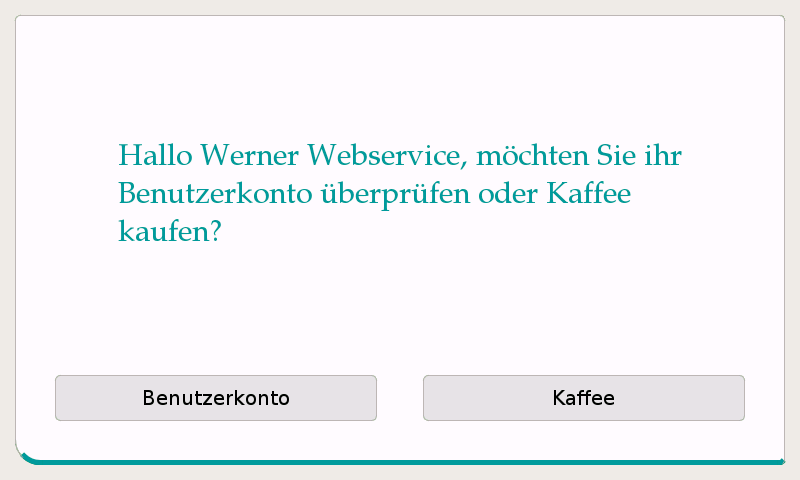
\includegraphics[width=.9\columnwidth]{images/screenshot}
    \caption{Grafische Oberfläche: Maske zur Aktionsauswahl durch den Benutzer.}
\end{figure}

Nach diesem Rückschlag wurde das QML-Konzept verworfen. Die Oberfläche wurde
mittels der Qt-Widgets-Bibliothek erstellt und läuft als Vollbild-Anwendung 
auf dem Raspberry Pi. In Abbildung \ref{fig:qt} ist die Maske zur Auswahl von
Aktionen durch den Benutzer nach erfolgter Authentifizierung dargestellt. Durch
die objektorientierte Schnittstelle von Qt, und dessen Möglichkeiten zur
Verwendung von Stylesheets, gelang die Entwicklung schnell. Als 
\glqq Eye-Candy\grqq{ }für die Nutzer konnten sogar Animationen bei den Übergängen von Ansicht
zu Ansicht eingebaut werden.

\subsection{Datenhaltung}

Zur Speicherung der Nutzerdaten wurde auf eine SQL-Datenbank zurückgegriffen.
Die Datenbank-Anbindung wurde mit dem Python-Paket
\emph{SQLAlchemy}\autocite{SQLAlchemy} realisiert. Es bietet einen komfortablen
Mapper von Python-Objekten nach Tabellen. 

Schwierigkeiten ergaben sich lediglich durch den Multi-Threading-Ansatz des 
Programmes, da so die gleichen Objekte in mehreren Datenbank-Sitzungen benötigt
wurden. Für diesen Fall bot sich die Verwendung von \texttt{scoped\_session}
an, die SQLAlchemy um eine thread-sichere Schnittstelle erweitert.

\section{Aktueller Stand und verpflichtende Features}

Zum gegenwärtigen Zeitpunkt sind die Grundfunktionalitäten des Projektes,
bestehend aus Ansteuerung der Hardware, Implementierung von zentralen 
Software-Komponenten, Datenbank-Anbindung und der grafischen Oberfläche 
erfolgt. Es fehlen nur noch zwei Komponenten zur Fertigstellung:

Eine Verwaltungsoberfläche für Administratoren muss noch implementiert werden.
Diese erlaubt es, den Kontostand beliebiger Nutzer am Gerät zu verändern, um
Einzahlungen in die Kaffeekasse zu ermöglichen. Auch das Anlegen/Entfernen
von Nutzern muss möglich sein.

Ein weiterer Punkt auf der TODO-Liste ist das Anfertigen eines Gehäuses für die
Kaffeekasse. Wegen der Größe des Bildschirms wird dieses vermutlich aus Holz
gefertigt werden, anstatt auf die beliebte 3D-Drucker-Lösung zurückzugreifen.

\section{Ausblick und Erweiterungsmöglichkeiten}

Mehrfach wurde vorgeschlagen, zur einfacheren Authentifizierung von Nutzern
einen \emph{Fingerabdruckleser} zu verwenden. Ein für DIY-Projekte gerne 
verwendeter günstiger Fingerabdruckleser befindet sich bereits im Besitz des
Autors. Die softwareseitige Einbindung sowie die Funktionsweise des Scanners
(Abspeicherung von Fingerabdrücken oder doch nur Hashwerten) muss jedoch noch
geklärt werden.

Auch die Ergänzung der grafischen Oberfläche durch die Anzeige von QR-Codes
ist gewünscht. Diese QR-Codes sollen Links zum Dienst \emph{Paypal me}
enthalten und so ein einfaches Bezahlen von aufgelaufenen Kaffee-Schulden
ermöglichen. Zu diesem Zweck sollen die Links mit den aktuellen Schulden
aus dem Benutzerkonto parametrisiert werden können.

Ein weiteres Wunsch-Feature ist die Abspeicherung von \emph{Transaktionen} mit
Zeitstempeln. Dies würde eine Analyse des persönlichen Kaffee-Konsums
ermöglichen. Die Implementierung dieses Features sollte als Opt-In nur für
interessierte Benutzer erfolgen. 

\printbibliography

\end{document}
